
\lecture{Correlation and Regression}{correlation-regression}
\section{Correlation and Regression}

\title{Correlation and Linear Regression}
\subtitle{Is a Straight Line Appropriate?}

%\author{Kelly Black}
%\institute{Clarkson University}
\date{15 April 2013}

\begin{frame}
  \titlepage
\end{frame}

\begin{frame}
  \frametitle{Outline}
  \tableofcontents[pausesection,hideothersubsections,sectionstyle=show/hide]
\end{frame}


\subsection{Clicker Quiz}

\iftoggle{clicker}{%
  \begin{frame}{Clicker Quiz}

    Determine if the following relationship is a ``positive relationship''
    or a ``negative relationship'' between the two variables.

    \begin{center}
      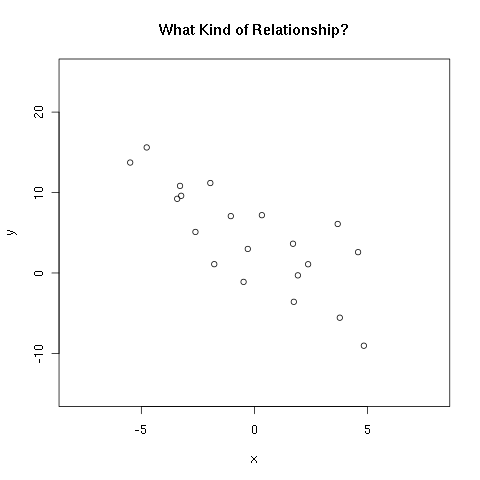
\includegraphics[width=6cm]{img/week2Day3ClickerQuizNeg}
    \end{center}

    \begin{tabular}{l@{\hspace{3em}}l}
      A: Positive & B: Negative
    \end{tabular}


  \end{frame}
}


\begin{frame}{Positive vs. Negative Relationships}

  \begin{columns}
    \column{.5\textwidth}
    Positive Relationship: \\
    \centerline{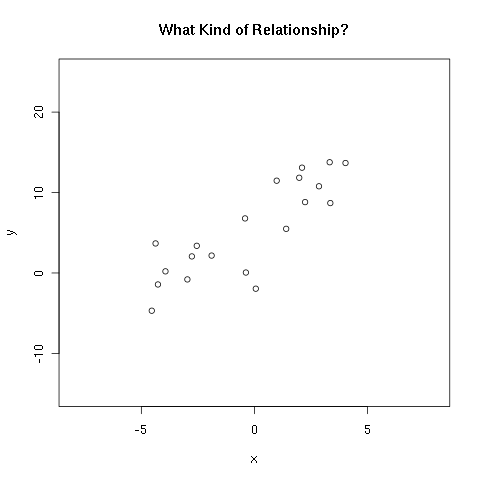
\includegraphics[width=5cm]{img/week2Day3ClickerQuizPos}}
    \column{.5\textwidth}
    Negative Relationship: \\
    \centerline{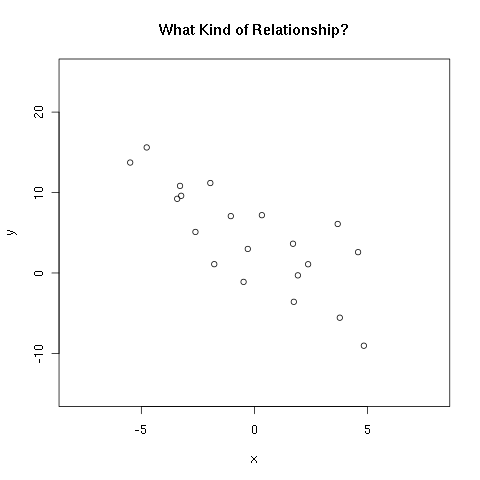
\includegraphics[width=5cm]{img/week2Day3ClickerQuizNeg}}
  \end{columns}
  
\end{frame}



\subsection{Correlation}

\begin{frame}{Correlation}

  \hspace*{-3em}
  \begin{tabular}{rrr}
    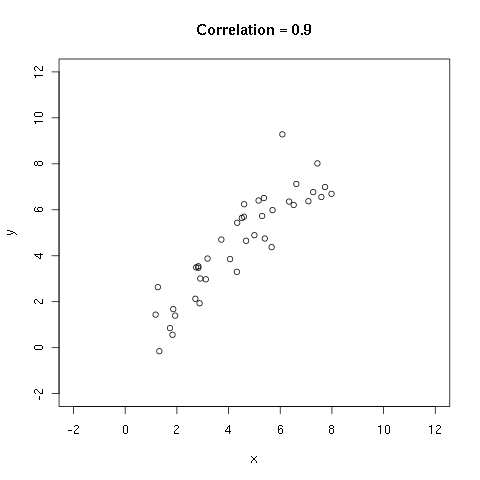
\includegraphics[height=4cm]{img/correlation09} & 
    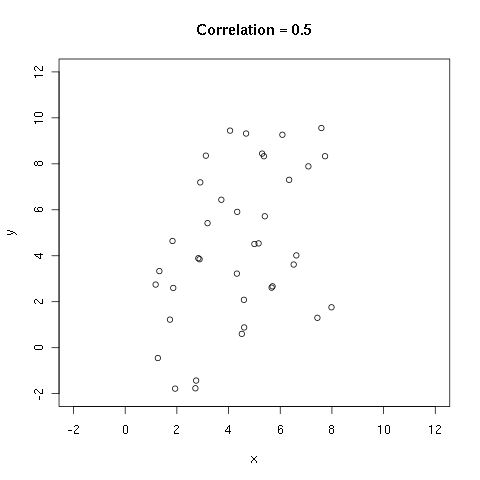
\includegraphics[height=4cm]{img/correlation05} &
    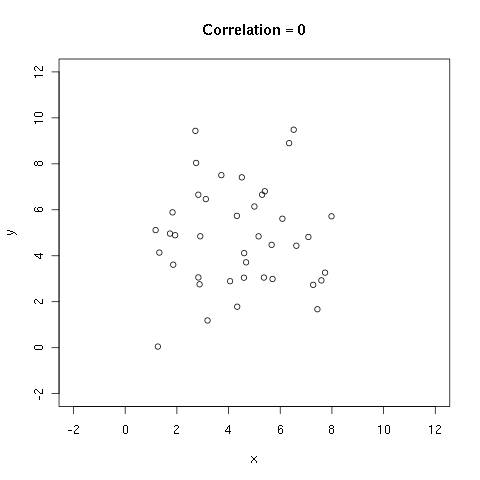
\includegraphics[height=4cm]{img/correlation0} \\
    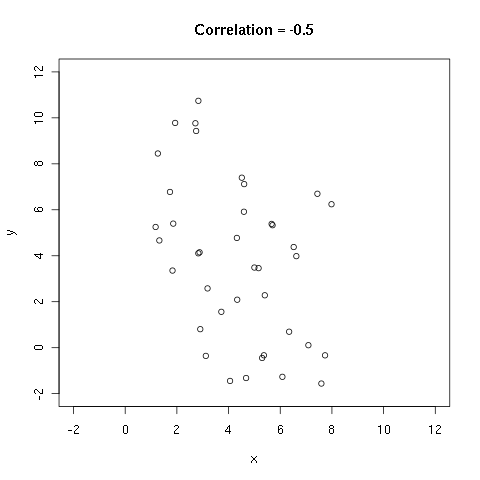
\includegraphics[height=4cm]{img/correlation-05} &
    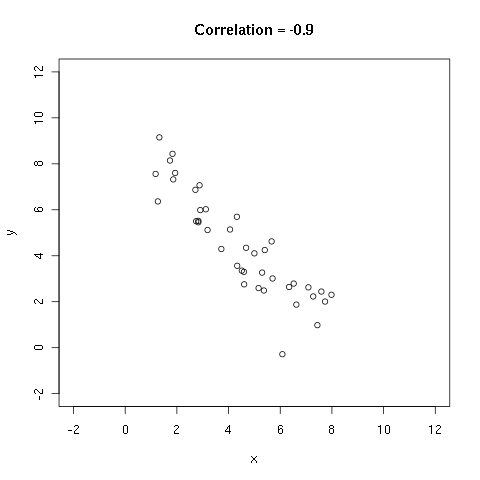
\includegraphics[height=4cm]{img/correlation-09}
  \end{tabular}


\end{frame}


\begin{frame}{Calculating the Correlation}

  First define the following sums:
  \begin{eqnarray*}
    S_{xx} & = & (x_1-\bar{x})^2 + (x_2-\bar{x})^2 + \cdot + (x_n-\bar{x})^2, \\
    S_{yy} & = & (y_1-\bar{y})^2 + (y_2-\bar{y})^2 + \cdot + (y_n-\bar{y})^2, \\
    S_{xy} & = & (x_1-\bar{x}) + (x_2-\bar{x}) + \cdot + (x_n-\bar{x}), \\
  \end{eqnarray*}

  \uncover<2->
  {
    
    \begin{definition}
      The sample correlation coefficient is defined to be
      \begin{eqnarray*}
        r & = & \frac{S_{xy}}{\sqrt{S_{xx} S_{yy}}}.
      \end{eqnarray*}
    \end{definition}

  }
  
\end{frame}



\begin{frame}{Example}
  
  \begin{columns}
    \column{.25\textwidth}
    \begin{tabular}{l|l}
      $x$ & $y$ \\ \hline
      -1 & -1 \\
      0 & 1 \\
      1 & 2 \\
      2 & 4
    \end{tabular}

    \column{.75\textwidth}
    
    \uncover<2->
    {
      \centerline{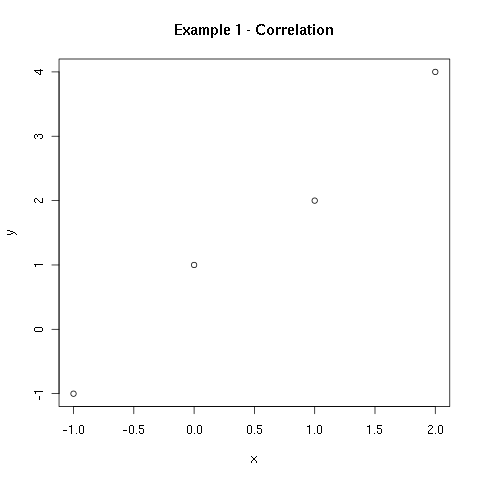
\includegraphics[width=6cm]{img/week2-Day3Correlation}}
    }

    \end{columns}

\end{frame}


\subsection{Linear Regression}



\iftoggle{clicker}{%
  \begin{frame}{Clicker Quiz}
  
    \begin{columns}
      \column{.25\textwidth}
      \begin{tabular}{r|r}
        $x$ & $y$ \\ \hline
        -1 & -1 \\
        0 & 1 \\
        1 & 2 \\
        2 & 4
      \end{tabular}

      \column{.75\textwidth}

      What is $S_{yy}$?

      \begin{tabular}{l@{\hspace{3em}}l@{\hspace{3em}}l@{\hspace{3em}}l}
        A: 5  & B: 8.5 & C: 13 & D: 16.75
      \end{tabular}

      \only<2->{%
        \begin{eqnarray*}
          \bar{y} & = & 1.5, \\
          s_{yy} & = & \lp -1 - 1.5\rp^2 + \lp 1 - 1.5\rp^2  + \\
                &   & \lp 2 - 1.5\rp^2 + \lp 4 - 1.5\rp^2 \\
                & = & 13
        \end{eqnarray*}
      }



    \end{columns}

  \end{frame}
}

\begin{frame}{Example}
  
  \begin{columns}
    \column{.25\textwidth}
    \begin{tabular}{r|r}
      $x$ & $y$ \\ \hline
      -1 & -1 \\
      0 & 1 \\
      1 & 2 \\
      2 & 4
    \end{tabular}

    \column{.75\textwidth}

    \only<1>{%
      \begin{eqnarray*}
        \bar{y} & = & 1.5, \\
        s_{yy}   & = & \lp -1 - 1.5\rp^2 + \lp 1 - 1.5\rp^2  + \\
                &   & \lp 2 - 1.5\rp^2 + \lp 4 - 1.5\rp^2 \\
                & = & 13, \\
        \bar{x} & = & 0.5 \\
        s_{xx}   & = & \lp -1 - 1.5\rp^2 + \lp 0 - 1.5\rp^2  + \\
                &   & \lp 1 - 1.5\rp^2 + \lp 2 - 1.5\rp^2 \\
                & = & 5, \\
        s_{xy}   & = & \lp -1 - 1.5\rp\lp -1 - 1.5\rp + \lp 0 - 1.5\rp\lp 1 - 1.5\rp  + \\
                &   & \lp 1 - 1.5\rp\lp 2 - 1.5\rp + \lp 2 - 1.5\rp\lp 4 - 1.5\rp \\
                & = & 8.
      \end{eqnarray*}
    }

    \only<2>{%
      \begin{eqnarray*}
        \bar{y} & = & 1.5, \\
        s_{yy}   & = & 13, \\
        \bar{x} & = & 0.5, \\
        s_{xx}   & = & 5, \\
        s_{xy}   & = & 8, \\
        r       & = & \frac{8}{\sqrt{5\cdot 13}}, \\
                & \approx & 0.99, \\
        \hat{m} & = & \frac{sxy}{sxx}= \frac{8}{5}, \\
        \hat{b} & = & \bar{y} - \hat{m} \bar{x} = 0.7.
      \end{eqnarray*}
    }

    \only<3->{%
      It is a positive relationship. As $x$ increases the value of $y$
      tends to increase.

      Question: What \textit{\color{red}percentage} of the change in
      $y$ is described by the change in $x$?

      \only<3>{\centerline{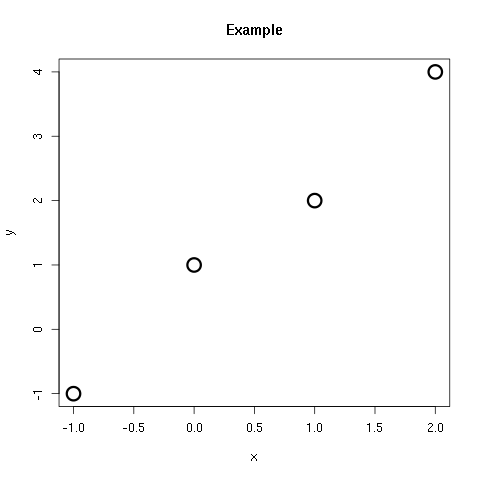
\includegraphics[width=5cm]{img/coefDetRaw}}}
      \only<4>{\centerline{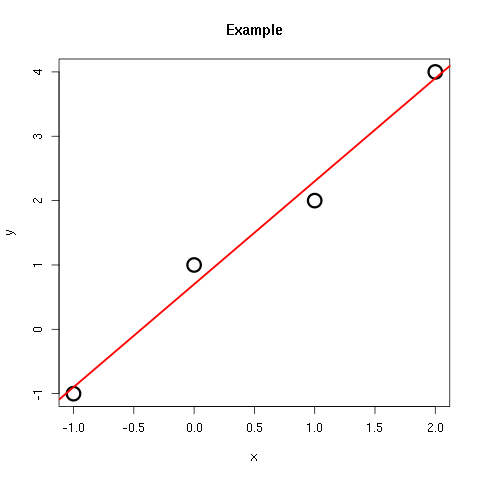
\includegraphics[width=5cm]{img/coefDetLine}}}
      %\begin{eqnarray*}
      %\end{eqnarray*}
    }


    \end{columns}

\end{frame}


\begin{frame}{Coefficient of Determination}

  Question: What \textit{\color{red}percentage} of the change in
  $y$ is described by the change in $x$?

  \centerline{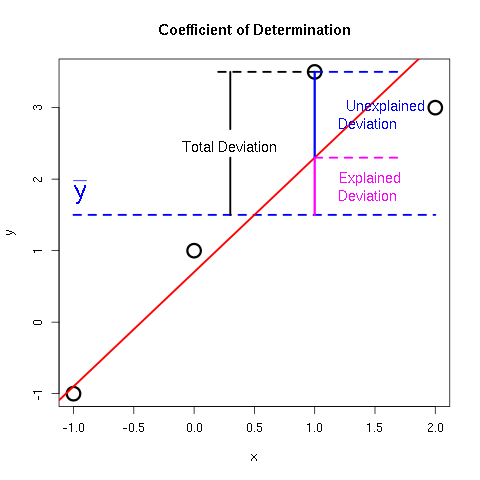
\includegraphics[width=5cm]{img/coefDetIdea}}

  \only<2->{%

    The coefficient of determination is the total percent of the
    deviation that is described by the linear regression line. It's
    value is $r^2$.

  }
  
\end{frame}

\begin{frame}{Example}
  
  \begin{columns}
    \column{.25\textwidth}
    \begin{tabular}{r|r}
      $x$ & $y$ \\ \hline
      -1 & -1 \\
      0 & 1 \\
      1 & 2 \\
      2 & 4
    \end{tabular}

    \begin{eqnarray*}
      r       & = & \frac{8}{\sqrt{5\cdot 13}}, \\
      & \approx & 0.99.
    \end{eqnarray*}


    \column{.75\textwidth}

    \centerline{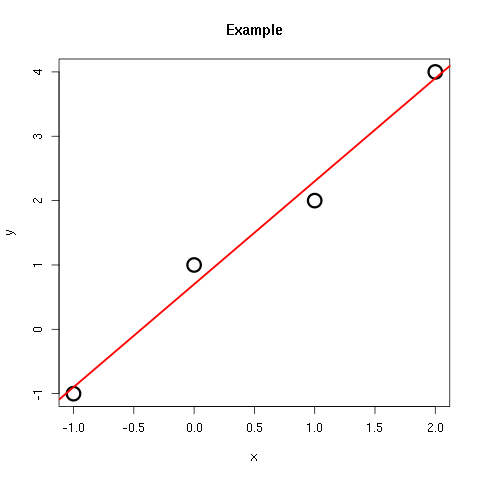
\includegraphics[width=4cm]{img/coefDetLine}}


    The coefficient of determination is
    \begin{eqnarray*}
      r^2 & = & \lp \frac{8}{\sqrt{5\cdot 13}} \rp^2, \\
      & \approx & 0.98.
    \end{eqnarray*}


    \end{columns}

\end{frame}


\begin{frame}{Example}
  
  \begin{columns}
    \column{.25\textwidth}
    \begin{tabular}{r|r}
      $x$ & $y$ \\ \hline
      -1 & -2 \\
      0 & 1 \\
      1 & 3 \\
      2 & 3
    \end{tabular}

    \only<4->{%

      \begin{eqnarray*}
        sxx & = & 5, \\
        syy & = & 16.75, \\
        sxy & = & 8.5.
        \only<5->{\\ r & = & \frac{8.5}{\sqrt{5\cdot 16.75}}.}
      \end{eqnarray*}

    }

    \column{.75\textwidth}
    
    \only<2>
    {
      \centerline{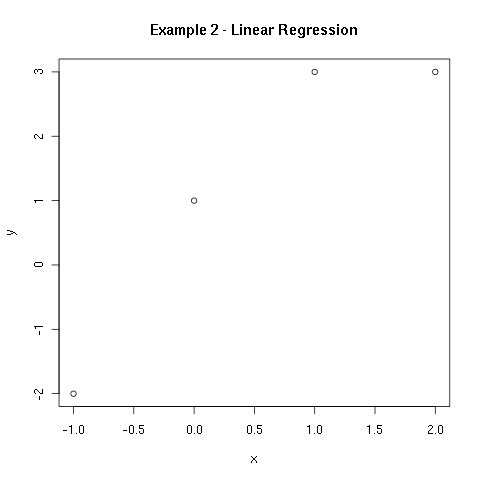
\includegraphics[width=5cm]{img/week2-Day3-Regression1}}
    }

    \only<3->
    {
      \centerline{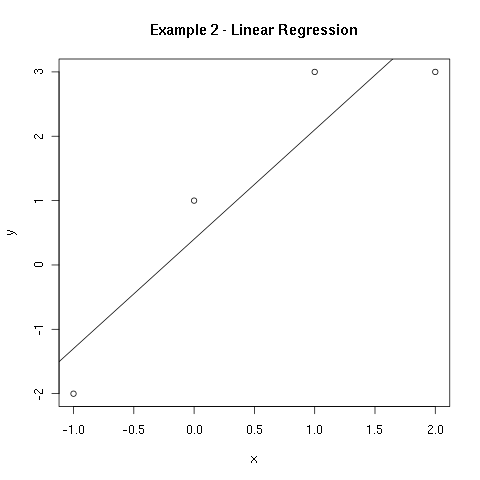
\includegraphics[width=5cm]{img/week2-Day3-Regression2}}
    }

    \only<4>
    {
      \begin{eqnarray*}
        r & = & \frac{8.5}{\sqrt{5\cdot 16.75}}.
      \end{eqnarray*}
    }

    \only<5->
    {
      \begin{eqnarray*}
        r^2 & = & \lp\frac{8.5}{\sqrt{5\cdot 16.75}}\rp^2, \\
          & \approx & 0.86
      \end{eqnarray*}
    }



    \end{columns}

\end{frame}



\begin{frame}{Clicker Quiz}

  What is the coefficient of determination for the following data?
  \begin{columns}
    \column{.25\textwidth}
    \begin{tabular}{r|r}
      $x$ & $y$ \\ \hline
      0 & 3 \\
      1 & 1.5 \\
      2 & 3 \\
      3 & 0
    \end{tabular}

    \begin{eqnarray*}
      sxx & = & 5.0, \\
      syy & = & 6.1875, \\
      sxy & = & -3.75.
      \only<5->{\\ r & = & \frac{8.5}{\sqrt{5\cdot 16.75}}.}
    \end{eqnarray*}

    \column{.75\textwidth}
    
    \centerline{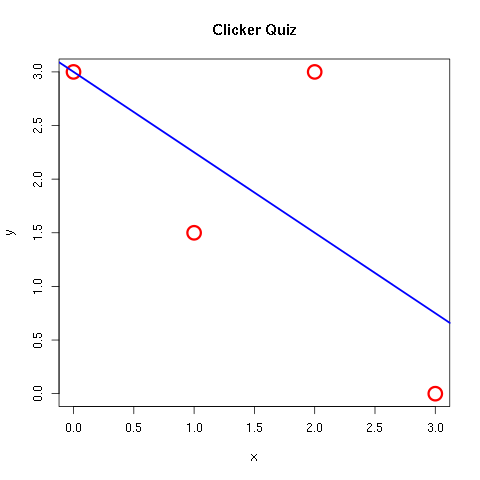
\includegraphics[width=5cm]{img/coefDetClickerQuiz}}

  \end{columns}

  \begin{tabular}{l@{\hspace{3em}}l@{\hspace{3em}}l}
    A: -0.67 & B: 0.67  & C: 0.45
  \end{tabular}

  
\end{frame}


% LocalWords:  Clarkson pausesection hideallsubsections rrr yy xy
